\documentclass{amsart}

\title{Based maps to Lagrangian Grassmanians, Quivers, and Bott Periodicity}
\author{Jim Bryan and Ravi Vakil}
\date{Last compiled:  \today.  Last edited:  December 12, 2024.}
\address{
Department of Mathematics\\
University of British Columbia \\
Room 121, 1984 Mathematics Road  \\
Vancouver, B.C., Canada V6T 1Z2  
}



\usepackage{diagbox}
\usepackage{float}
\usepackage{graphicx}
\usepackage{booktabs}
\usepackage{amsmath}
\usepackage{bm}
%\usepackage{pict2e,keyval,calc,fp}
%\usepackage{etex}
\usepackage{verbatim}
\usepackage{amsmath,amsthm,amsfonts}
\usepackage{amssymb}
\usepackage{times}
\usepackage{longtable}
\usepackage{caption}
\usepackage{array}
\usepackage{tikz-cd}
\usepackage{mathtools}
%\usepackage{amstex}
%\linespread{1.1}
\usepackage{tikz}
\usetikzlibrary{arrows,positioning}


\newtheorem{theorem}{Theorem}[section]
\newtheorem{proposition}[theorem]{Proposition}
\newtheorem{conjecture}[theorem]{Conjecture}
\newtheorem{lemma}[theorem]{Lemma}
\newtheorem{corollary}[theorem]{Corollary}
\newtheorem{convention}{Convention}[theorem]
\newtheorem{case}{Case}[theorem]
%\numberwithin{case}{theorem}


\theoremstyle{definition}

\newtheorem{remark}[theorem]{Remark}
\newtheorem{def-theorem}[theorem]{Definition-Theorem}
\newtheorem{definition}[theorem]{Definition}
\newtheorem{example}[theorem]{Example}
\newtheorem{assumption}[theorem]{Assumption}
\newtheorem{expectation}[theorem]{Expectation}





\usepackage{amsmath}
\usepackage{amsmath,amsthm,amsfonts}
\usepackage{times}
%\usepackage{amstex}

\newcommand{\smargin}[1]{\marginpar{\tiny{#1}}}

\newcommand{\CC} {{\mathbb C}}          % complex numbers
\newcommand{\NN} {{\mathbb N}}		% natural numbers
\newcommand{\RR} {{\mathbb R}}		% real numbers
\newcommand{\ZZ} {{\mathbb Z}}		% integers
\newcommand{\QQ} {{\mathbb Q}}		% rationals
\newcommand{\FF} {{\mathbb F}}
\newcommand{\evir}{e_{\mathsf{vir}}}
\newcommand{\reg}{\mathsf{reg}}
\newcommand{\calE}{\mathcal{E}}






\newcommand{\PP}{\mathbb{P}}
\newcommand{\OO}{\mathcal{O}}
\newcommand{\M}{{\mathsf{M}}}


\newcommand{\tinyhalf}{\tfrac{1}{2}}

\newcommand{\Hom}{\operatorname{Hom}}
\newcommand{\Ker}{\operatorname{Ker}}
\newcommand{\End}{\operatorname{End}}
\newcommand{\Ext}{\operatorname{Ext}}
\newcommand{\Tr}{\operatorname{tr}}
\newcommand{\tr}{\operatorname{tr}}
\newcommand{\Coker}{\operatorname{Coker}}
\newcommand{\coker}{\operatorname{coker}}
\newcommand{\im}{\operatorname{Im}}
\newcommand{\Km}{\operatorname{Km}}
\newcommand{\Fun}{\operatorname{Fun}}
\newcommand{\Sym}{\operatorname{Sym}}
\newcommand{\NS}{\operatorname{NS}}
\newcommand{\Pic}{\operatorname{Pic}}
\newcommand{\Coef}{\operatorname{Coef}}
\newcommand{\Isom}{\operatorname{Isom}}
\newcommand{\Hilb}{\operatorname{Hilb}}
\newcommand{\Tot}{\operatorname{Tot}}
\newcommand{\UL}[1]{\underline{#1}}
\newcommand{\alg}{\mathsf{alg}}
\newcommand{\stable}{\mathsf{s}}
\renewcommand{\top}{\mathsf{top}}
\newcommand{\Gr}{\operatorname{Gr}}
\newcommand{\LGr}{\operatorname{LGr}}
\newcommand{\OGr}{\operatorname{OGr}}
\newcommand{\LoopTwo}{\Omega^{2}_{d,\alg}}
\newcommand{\LoopTwoTop}{\Omega^{2}_{d,\top}}
\newcommand{\NoDLoopTwo}{\Omega^{2}_{\alg}}
\newcommand{\NoDLoopTwoTop}{\Omega^{2}_{\top}}
\newcommand{\Id}{\operatorname{Id}}
\newcommand{\codim}{\operatorname{codim}}
\newcommand{\homotopyeq}{\simeq}


\begin{document}

\begin{abstract}
We give a quiver description of the space of based algebraic maps from
$\PP^{1}$ to the Lagrangian Grassmanian (and its orthogonal
counterpart). Combined with a result of Mann-Milgram, we get new proof of some
of the homotopy equivalences in orthogonal Bott periodicity.
\end{abstract}

\maketitle 

\markboth{Short title 1}  {Short title 2}
%\renewcommand{\sectionmark}[1]{}


%\tableofcontents
%\pagebreak

\section{Introduction}\label{sec: intro}


\subsection{Algebraic and Topological double loop spaces and Bott periodicity.}

In this paper, we study the \emph{algebraic double loop space} of
Lagrangian Grassmannians and the orthogonal counter part. The
algebraic double loop space is defined as follows.

\begin{definition}\label{defn: Omega2alg(X)}
Let $(X,*)$ be a variety with a base point $*\in X$. Fix homogeneous
coordinates $(x_{0}:x_{1})$ on $\PP^{1}$ with point at infinity
$p_{\infty}=(1:0)$. Let $\LoopTwo(X)$ be the space algebraic based
maps of degree $d$, that is
\[
\LoopTwo (X) = \left\{f:\PP^{1}\to X\text{ such that
$f(p_{\infty})=*$ and $f_{*}([\PP^{1}])=d\in H_{2}(X,\ZZ )$. } \right\} .
\]
\end{definition}

In the analytic topology over $\CC$, $\PP^{1}$ is homeomorphic to
$S^{2}$ and so there is an inclusion of the algebraic double loop
space into the usual double loop space studied in topology:
\[
i:\LoopTwo (X) \hookrightarrow \LoopTwoTop (X)
\]
where $\LoopTwoTop (X)$ is the space of continuous based maps of
degree $d$ (we will drop the $d$ from the notation when $H_{2}(X)=0$).

In the same spirit as using high degree polynomial functions to
approximate a continuous function, we may hope that for certain
varieties $X$, the algebraic loop space approximatees the topological
loop space in the sense that it captures most of its homotopy theory.

\begin{expectation}
For certain varieties $X$, $i:\LoopTwo (X) \hookrightarrow \LoopTwoTop
(X)$ is a \emph{homotopy approximation} meaning that 
\[
i_{*}:\pi_{k}(\LoopTwo (X)) \to \pi_{k}( \LoopTwoTop (X))
\]
is an isomorphism for all $k<B(d,X)$ and that $B\to \infty $ as $d\to
\infty$. 
\end{expectation}

In the 1980's and 1990's the above expectation was shown to hold for
generalized flag varieties in a series of papers by Kirwan, Segal, and
Mann-Milgram \cite{???,???,???}

\begin{theorem}\label{thm: Mann-Milgram algebraic loop approximation
holds for generalized flag varieties}
Let $G$ be a reductive algebraic group over $\CC$, let $P\subset G$
be a parabolic subgroup, and let $X=G/P$ be the corresponding
generalized flag variety. Then the above expectation holds.
\end{theorem}

The (topological) double loop space $\LoopTwoTop (X)$ plays an
important role in homotopy theory, for example in Bott periodicity. To
state the version of Bott periodicity we want, we recall that $U(n)$,
$Sp(2n)$, and $O(2n)$ are the classical compact Lie groups of unitary,
symplectic, and orthogonal transformations. We also have the infinite
dimensional versions of these groups (definied by direct limits of
inclusions) and their associated classifying spaces and homogeneous
spaces. For example:
\begin{align*}
U&=\lim_{n\to  \infty} U(n),\\
Sp/U& = \lim_{n\to  \infty} Sp(2n)/U(n),\\
BO& = \lim_{n\to  \infty} BO(n),\\
\end{align*}
and so forth.

One version of Bott periodicity is tehn given as follows.

\begin{theorem}\label{thm: classical Bott periodicity as homotopy equivalences}
There exist the following homotopy equivalences:
\begin{align}
\LoopTwoTop (BU)&\homotopyeq BU \label{eqn: Omega2BU=BU}\\
\LoopTwoTop (SP/U)&\homotopyeq BO  \label{eqn: Omega2Sp/U=BO}\\
\NoDLoopTwoTop (BO)&\homotopyeq O/U  \label{eqn: Omega2BO=O/U}\\
\LoopTwoTop (O/U)&\homotopyeq BSp  \label{eqn: Omega2O/U=BSp}\\
\NoDLoopTwoTop (BSp)&\homotopyeq Sp/U   \label{eqn: Omega2BSp=Sp/U}
\end{align}
\end{theorem}

Equation~\eqref{eqn: Omega2BU=BU} is referred to as \emph{complex Bott
periodicity} and it implies that the homotopy groups of $U$ are
2-periodic. Equations~\eqref{eqn: Omega2Sp/U=BO}-\eqref{eqn: Omega2BSp=Sp/U} 
are referred to as \emph{real Bott periodicity} and they imply that
the homotopy groups of $O$ are 8-periodic.

\subsection{Summary of main results}

The main results of this paper give explicit descriptions of $\LoopTwo
(X)$ when $X$ is a Grassmanian, a Lagrangian Grassmanian, or an
isotropic orthogonal Grassmanian. Our description is in terms of
moduli spaces of quiver representations. We use our descriptions along
with Theorem~\ref{thm: Mann-Milgram algebraic loop approximation
holds for generalized flag varieties} to give new proofs of the
homotopy equivalences \eqref{eqn: Omega2BU=BU}, \eqref{eqn:
Omega2Sp/U=BO}, and \eqref{eqn: Omega2O/U=BSp} and so we may regard
our theorems as finite dimensional, algebraic refinements of Bott
periodicity. The study of the remaining equivalences in the Bott
periodicity theorem from the perspective of this paper will be pursued
in future work.

To state our results more explicitly, let $\Gr(n,n+N)$ be the
Grassmanian of $n$ dimensional quotients of a fixed $n+N$ dimensional
vector space.  Let $\LGr (n,2n)$ (respectively $\OGr (n,2n)$) be the
Lagrangian (respectively isotropic orthogonal) Grassmanian which
parameterizes $n$ dimensional isotropic  quotients of a fixed $2n$
dimensional vector space equipped with a symplectic (respectively
orthogonal) bilinear form. For $X$ given by $\Gr (n,n+N)$, $\LGr
(n,2n)$, or $\OGr (n,2n)$, $H_{2}(X)\cong \ZZ$ as so the class of a
map $f:\PP^{1}\to X$ may be regarded as a positive integer (the
degree).


\begin{theorem}\label{thm: quiver description of Loop2alg(Gr(n,n+N))}
Let $A$ be a vector space of dimension $d$ and let $U,W$ be vector
spaces of dimension $n$ and $N$ respectively. Let
\[
V=V_{n,N,d} =\Hom (A,A)\oplus \Hom (W,A)\oplus \Hom (A,U).
\]
Then $GL(A)$ acts naturally on $V$ and let $V^{\stable}\subset V$ be
the locus of stable points in the sense of GIT. Then there exists a
natural isomorphism:
\[
\LoopTwo (\Gr (n,n+N))\cong V^{\stable}/GL(A).
\]
\end{theorem}

For the Lagrangian and isotropic orthogonal Grassmannians we have the following.

\begin{theorem}\label{thm: quiver description of Loop2Alg(LGr)}
Let $A$ be a vector space of dimension $d$ equipped with a
non-degenerate orthogonal form $\phi :A\to A^{\vee}$ (so
$\phi^{\vee}=\phi$) and let $U$ be a vector space of dimension
$n$. Let
\[
V=V_{n,d}=\left\{(\alpha ,j)\in \Hom (A,A)\oplus \Hom (A,U):
\alpha^{\vee}\phi =\phi \alpha \right\} 
\]
and let 
\[
O(A,\phi ) = \left\{g\in GL(A):g^{\vee}\phi g=\phi  \right\}
\]
be the group of orthogonal isomorphisms of $A$. Then $O(A,\phi )$ acts
naturally on $V$ and let $V^{\stable}\subset V$ be the stable
locus (in the sense of GIT). Then
\[
\LoopTwo (LG(n,2n))\cong V^{\stable}/O(A,\phi ). 
\]
\end{theorem}

The statement for the isotropic orthogonal Grassmannian is similar:


\begin{theorem}\label{thm: quiver description of Loop2Alg(OGr)}
Let $A$ be a vector space of dimension $d$ equipped with a
non-degenerate symplectic form $\phi :A\to A^{\vee}$ (so
$\phi^{\vee}=-\phi$) and let $U$ be a vector space of dimension
$n$. Let
\[
V=V_{n,d}=\left\{(\alpha ,j)\in \Hom (A,A)\oplus \Hom (A,U):
\alpha^{\vee}\phi =\phi \alpha \right\} 
\]
and let 
\[
Sp(A,\phi ) = \left\{g\in GL(A):g^{\vee}\phi g=\phi  \right\}
\]
be the group of symplectic isomorphisms of $A$. Then $Sp(A,\phi )$ acts
naturally on $V$ and let $V^{\stable}\subset V$ be the stable
locus (in the sense of GIT). Then
\[
\LoopTwo (OG(n,2n))\cong V^{\stable}/Sp(A,\phi ). 
\]
\end{theorem}

The quivers associated to our theorems are given in the following figure:

\begin{center}
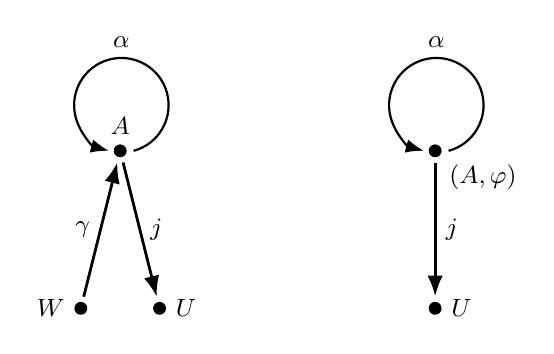
\begin{tikzpicture}

\tikzset{myarrow/.style={-Latex, thick,line width=1pt,shorten >=2pt, shorten <=2pt}}

    % Node positioning
    \def\yDist{1.0} % Vertical distance between nodes
    \def\loopRadius{0.6} % Radius of the loop circles

    % Left quiver
    \node[draw, circle, fill, inner sep=1.5pt, label=above:{\small
    $A$}] (L1) at (-2,\yDist) {}; 
    \node[draw, circle, fill, inner sep=1.5pt, label=right:{\small
    $U$}] (L2) at (-1.5,-\yDist) {}; 
    \node[draw, circle, fill, inner sep=1.5pt, label=left:{\small
    $W$}] (L3) at (-2.5,-\yDist) {}; 
    \draw[myarrow] (L1) -- node[right] {\small $j$} (L2);
    \draw[myarrow] (L3) -- node[left] {\small $\gamma $} (L1);

    % Loop for left node
     \draw[-Latex,thick] (-1.83,\yDist) arc (-75:255:\loopRadius) node[midway,
     above] {\small $\alpha$}; 

    % Right quiver
    \node[draw, circle, fill, inner sep=1.5pt, label=below right:{\small
    $(A,\varphi)$}] (R1) at (2,\yDist) {}; 
    \node[draw, circle, fill, inner sep=1.5pt, label={right:{\small
    $U$}}] (R2) at (2,-\yDist) {}; 
    \draw[myarrow] (R1) -- node[right] {\small $j$} (R2);

    % Loop for right node
     \draw[-Latex,thick] (2.17,\yDist) arc (-75:255:\loopRadius) node[midway,
     above] {\small $\alpha$}; 

\end{tikzpicture}
\end{center}

\subsection{Topological Consequences}\label{subsec: topological consequences}

In this section we explain how our quiver descriptions of $\LoopTwo
(OG(n,2n))$ and $\LoopTwo (LG(n,2n))$  lead to proofs of the Bott
periodicity equivalences given by eqns~\eqref{eqn: Omega2O/U=BSp} and
\eqref{eqn: Omega2Sp/U=BO} respectively.


\begin{definition}\label{defn: homotopy approximation}
We say a collection of topological spaces $\{X_{d} \}_{d\in \NN }$ is
a \emph{homotopy approximation} for a topological space $Y$ if there
are bounds $B_{d}\in \NN $ and maps $f_{d}:X_{d}\to Y$ which induce
isomorphisms 
\[
(f_{d})_{*}:\pi_{k}(X_{d})\to \pi_{k}(Y)
\]
for all $k<B_{d}$ and $\lim_{d\to \infty}B_{d} = \infty$. Moreover we
assume there are maps $i_{d}:X_{d}\to X_{d+1}$ which commute with the
$f_{d}$s and that $X_{d}$ have the homotopy type of a CW complex. We
denote homotopy approximation as follows:
\[
\{X_{d} \}\homotopyeq_{d} Y.
\]
\end{definition}

The definitions, along with the Whitehead theorem imply that if
$\{X_{d} \}\homotopyeq_{d} Y$, then $Y\homotopyeq \lim_{d\to
\infty}X_{d}$.

The two examples of homotopy approximation relavant to the paper are
the following.
\subsubsection{Mann-Milgram Homotopy approximation}\label{subsubsec:
Mann-Milgram homot approx}
We note that unlike the algebraic double loop spaces, the topological
double loop spaces of each degree are all homotopic:
\[
\LoopTwoTop (X)\homotopyeq \Omega^{2}_{0,\top}(X).
\]
Then Theorem \ref{thm: Mann-Milgram algebraic loop approximation
holds for generalized flag varieties} says that 
\[
\{\LoopTwo (X) \}\homotopyeq_{d}  \Omega^{2}_{0,\top}(X).
\]
if $X$ is a generalized flag variety, in particular, if $X$ is
$Gr(n,n+N)$, $LGr(n,2n)$, or $OGr(n,2n)$.

\subsubsection{GIT homotopy approximation}\label{subsubsec: GIT
homotopy approx}



\vfill
\pagebreak


On the subsequent pages are old sections that we can either incorporate or not.        

\vfill
\pagebreak


\section{Temporary notation section}

This section is just so we have our notation that we are fixing once and for all.

$x_0$, $x_1$ are projective coordinates on $\PP^1$.

\section{A Retelling of Larson-Vakil}

This section probably won't end up in the paper. The purpose here is
to use it as the prototype for the way we treat the 8-fold case and to
fix some ideas and notation.

\subsection{Notation and Definitions}

We fix homogeneous coordinates $(x_{0}:x_{1})$ on $\PP^{1}$ and we let
$p_{\infty }=(1:0)$. Let $V$ be a vector space. We use the notation
\[
\UL{V}(k) = \OO_{\PP^{1}}(k)\otimes V.
\]

\begin{definition}\label{defn: Omega2alg}
Let $(X,\bullet )$ be a (quasi-projective) variety with a base point
$\bullet \in X$. We define the algebraic loop-2 space of $X$ by
\[
\LoopTwo (X) = \left\{f:\PP^{1}\to X \quad :\quad
f(p_{\infty})=\bullet , f_{*}([\PP^{1}])=d\in A_{1}(X) \right\}.
\]
\end{definition}


Let $U$ and $W$ be vector spaces of dimension $n$ and $N$ respectively
and let
\[
\Gr (n,n+N) = \Gr (n,U\oplus W)
\]
be the Grassmannian of $n$ dimensional quotients of $U\oplus W$ with
basepoint given by the projection $U\oplus W\to U$. By pulling back
the universal quotient, we see that $\LoopTwo (\Gr (n,n+N))$
parameterizes exact sequences:

\[
\begin{tikzcd}
0\arrow[r]& F \arrow[r]& \UL{U}\oplus \UL{W} \arrow{r}{\theta } &E
\arrow[r]& 0
\end{tikzcd}
\]
where $E$ is a rank $n$, degree $d$ bundle on $\PP^{1}$ and
$E|_{p_{\infty}}\cong U$ via the first component of $\theta
=({\UL{\theta}_U},\UL{\theta}_{W})$ and where the map
\[
\UL{\theta }_{{W}}:\UL{W}\to E
\]
is zero at $p_{\infty}$ and hence
factors through a map
\[
\UL{\gamma} :\UL{W} \to E(-p_{\infty}).
\]

Since $E$ is a quotient of a trivial bundle, it is non-negative in the
following sense:
\begin{definition}
A vector bundle $E$ on $\PP^{1}$ is non-negative (respectively
positive, less than $k$, etc.) if its splitting type $E\cong
\oplus_{i}\OO (a_{i})$ satisfies $a_{i} \geq 0$ (respectively
$a_{i}>0$, $a_{i}<k$, etc.) for all $i$. 
\end{definition}


Because $E$ is non-negative, the sheaf map $\UL{\theta}_{U}$ is
determined by its map on global sections which we denote without the
underline:
\[
\theta_{U}:U \longrightarrow H^{0}(E).
\]
Then the exact sequence
\[
\begin{tikzcd}
0\arrow[r]&E(-p_{\infty})\arrow{r}{\cdot \UL{x}_{1}}
&E\arrow[r]&E|_{p_{\infty}} \arrow[r] &0
\end{tikzcd}
\]
induces a sequence
\[
\begin{tikzcd}
0\arrow[r]&H^{0}(E(-p_{\infty}))\arrow{r}{\cdot {x}_{1}}
&H^{0}(E)\arrow[r]&U \arrow[r] &0
\end{tikzcd}
\]
which is split by $\theta_{U}:U\to H^{0}(E)$ inducing the isomorphism
\[
H^{0}(E) = A\oplus U
\]
where 
\[
A=H^{0}(E(-p_{\infty}))
\]
is a vector space of dimension $d$.

Then the sheaf map
\[
\begin{tikzcd}
 E(-p_{\infty})\arrow{r}{\cdot \UL{x}_{0}} &E
\end{tikzcd}
\]
induces a map in cohomology
\[
\begin{tikzcd}
A\arrow{r}{\cdot x_{0}} &A\oplus U
\end{tikzcd}
\]
whose components we denote by $\alpha$ and $j$:
\[
\alpha :A\to A, \quad j: A\to U.
\]
Finally, the sheaf map
\[
\begin{tikzcd}
\UL{W}\arrow{r}{\UL{\gamma}} & E(-p_{\infty})
\end{tikzcd}
\]
is determined by its map in cohomology
\[
\gamma :W\to A.
\]


\subsection{The main result}
With the notation of the previous subsection we can now state the main
geometric result of this section.

\begin{theorem}\label{thm: quiver description of loop2 of Gr}
Let $U$, $W$, and $A$ be vector spaces of dimension $n$, $N$, and
$d$. Let $V = \Hom (A,A)\oplus \Hom (A,U)\oplus \Hom (W,A)$ and let
$V^{0}\subset V$ be the open set of $(\alpha ,j,\gamma )\in V$
satisfying
\begin{enumerate}
\item $\Ker (\alpha -\lambda \cdot \Id_{A})\cap \Ker (j) = 0$ for all
$\lambda$.
\item  $\im (\alpha -\lambda \cdot \Id_{A})+ \im (\gamma )=A$ for
all $\lambda$.
\end{enumerate}
Then the constructions of the previous subsection induce an
isomorphism of affine varieties:
\[
\LoopTwo (\Gr (n,n+N))\cong V^{o}/GL(A) .
\]
\end{theorem}
\begin{remark}\label{rem: Gr(n,n+N) is a model for BGL(n) and Vo/GL(A) is a model for BGL(d)}
The Grassmannian on the left is an approximate model for $BGL(n)$ and
the quotient on the right is an approximate model for $BGL(d)$. We can
thus regard our theorem as saying, in a sense that we will make
precise in the next subsection, that there is an approximate
equivalence $\Omega^{2}(BGL(n))\sim BGL(d)$.
\end{remark}

\begin{remark}\label{rem: duality induced by Gr(n,n+N)=Gr(N,n+N)}
The isomorphism $\Gr (n,U\oplus W)\cong \Gr (N,U^{\vee}\oplus
W^{\vee})$ given by dualizing exact sequences induces an isomorphism
on the quiver side given by $(A,U,W)\mapsto
(A^{\vee},W^{\vee},U^{\vee})$ and $(\alpha ,j,\gamma )\mapsto
(\alpha^{\vee},\gamma^{\vee},j^{\vee})$. Note that the two open
conditions (1) and (2) are dual to each other under this equivalence. 
\end{remark}



To prove the theorem we begin with the following
\begin{lemma}\label{lem: Stromme}
Let $E$ be a non-negative bundle on $\PP^{1}$. Then the following
sequence is exact:
\[
\begin{tikzcd}
0\arrow{r} & \UL{H^{0}(E(-1))}(-1)
\arrow{rr}{\UL{x}_{1}x_{0}-\UL{x}_{0}x_{1}}& &
\UL{H^{0}(E)} \arrow{r} & E\arrow[r] & 0
\end{tikzcd}
\]
where as in the previous section, sheaf maps are denoted with
underlines and their induced maps on cohomology are denoted without,
so in particular $\UL{x}_{i}:\OO (-1)\to \OO$ and
$x_{i}:H^{0}(E(-1))\to H^{0}(E)$ in the above.
\end{lemma}
\begin{proof}
Let $\PP^{1}\times \PP^{1}$ have coordinates
$((y_{0}:y_{1}),(x_{0}:x_{1}))$ with $p,q:\PP^{1}\times \PP^{1}\to
\PP^{1}$ projection onto the first and second factor respectively. Let 
\[
\Delta =\{y_{1}x_{0}-y_{0}x_{1} =0 \}\subset \PP^{1}\times \PP^{1}
\]
be the diagonal. Then we get an isomorphism
\[
E\cong q_{*}\left(p^{*}E\otimes \OO_{\Delta} \right)
\]
where we have implicitly identified the two factors of $\PP^{1}$ by
$x_{i}=y_{i}$.  We then tensor the exact sequence
\[
\begin{tikzcd}
0\arrow[r] & \OO_{\PP^{1}\times \PP^{1}}(-1,-1)
\arrow{rr}{y_{1}x_{0}-y_{0}x_{1}}& & \OO_{\PP^{1}\times \PP^{1}}
\arrow[r]& \OO_{\Delta} \arrow[r]& 0
\end{tikzcd}
\]
by $p^{*}E$ and apply the functor $q_{*}(-)$. Since the non-negativity
of $E$ implies that $R^{1}q_{*}(p^{*}E(-1,-1))=0$, we get
\[
\begin{tikzcd}
0\arrow[r] &q_{*}(p^{*}E(-1,-1)) \arrow[r] & q_{*}(p^{*}E) \arrow[r] &
q_{*}(p^{*}(E))\otimes \OO_{\Delta} \arrow[r] & 0 
\end{tikzcd}
\]
which can be written as 
\[
\begin{tikzcd}
0\arrow[r] &\UL{H^{0}(E(-1))}(-1)
\arrow{rr}{\UL{y_{1}}x_{0}-\UL{y_{0}}x_{1}} && \UL{H^{0}(E)} \arrow[r]
&E \arrow[r] &0
\end{tikzcd}
\]
which proves the lemma.
\end{proof}

Now let 
\[
\UL{U} \oplus \UL{W} \to E \to 0
\]
be a point in $\LoopTwo (\Gr (n,n+N))$ and recall that 
\[
x_{0},x_{1}: H^{0}(E(-p_{\infty})) \to H^{0}(E)
\]
are given by
\[
\begin{tikzcd}
A \arrow{r}{\begin{pmatrix} \alpha \\ j  \end{pmatrix}} &A\oplus U,
\quad & A \arrow{r}{\begin{pmatrix} \Id_{A} \\ 0  \end{pmatrix}} &A\oplus U
\end{tikzcd}
\]
respectively. Then the exact sequence from Lemma~\ref{lem: Stromme}
reads
\[
\begin{tikzcd}
0 \arrow[r] &\UL{A}(-1) \arrow{rr}{\begin{pmatrix} \UL{x}_{1}\alpha -\UL{x}_{0}\\
\UL{x}_{1}j  \end{pmatrix}}&&\UL{A}\oplus \UL{U}\arrow[r]&E
\arrow[r]& 0.
\end{tikzcd}
\]

The condition that $\UL{A}(-1)$ is a subbundle of $\UL{A}\oplus
\UL{U}$ requires that for any point $\lambda =\frac{x_{0}}{x_{1}}\in
\PP^{1}-p_{\infty}$, the vector space map ${\tiny \begin{pmatrix} \alpha -\lambda \Id_{A}\\
j \end{pmatrix}} : A\to A\oplus U $ is injective. This is equivalent
to condition (1) of the theorem.

The condition that $\theta :\UL{U}\oplus \UL{W} \to E$ is surjective
means that the map 
\[
\UL{W} \to Q
\]
is surjective where $Q$ is the rank zero sheaf given by the cokernal
of $\UL{\theta}_{U}$:
\[
\begin{tikzcd}
0\arrow[r]& \UL{U} \arrow{r}{\UL{\theta}_{U}} & E\arrow[r]&Q\arrow[r]&0.
\end{tikzcd}
\]
The cohomology exact sequence of the above canonically identifies
$A\cong H^{0}(Q)$ and under this identification, the map in cohomology
induced by $\UL{W}\to Q$ is just $\gamma :W\to A$.

\emph{Sketchy completion of this argument:}  The support of $Q$ is
given by the eigenvalues of $\alpha$ so $\UL{W}\to Q$ being surjective
is equivalent to $\gamma$ surjecting onto the eigenspaces of $\alpha$
which is exactly condition (2) of the theorem. This more or less finishes up the
proof of the theorem. I guess I haven't said very carefully that the
point in $\LoopTwo (\Gr (n,n+N))$ is uniquely determined by $(\alpha
,j,\gamma )$ up to the action of $GL(A)$ although it is implicit in
the above argument. Also needed: prove that the quotient $V^{o}/GL(A)$
is an affine variety (it is an affine GIT  quotient). \emph{Is this
even true? I think it is.}


\subsection{Topological consequences of the theorem}\label{subsec:
topological consequences}

In this subsection, we make precise the assertion in Remark~\ref{rem:
Gr(n,n+N) is a model for BGL(n) and Vo/GL(A) is a model for
BGL(d)}. We work over $\CC$ and we give our varieties the analytic
topology. Then since $\PP^{1}$ is homeomorphic to the 2-sphere
$S^{2}$, there is a natural inclusion
\[
\LoopTwo (\Gr (n,n+N))\hookrightarrow \LoopTwoTop  (\Gr (n,n+N))
\]
where the space on the right is the usual loop-2 space of continuous
based maps $f:S^{2}\to \Gr (n,n+N)$.

In \cite{Mann-Milgram-93}, Mann and Milgram study the above inclusion
and prove that it induces a homotopy equivalence through dimension
$2d+1$ (and that moreover this bound is sharp). In other words we have
an isomorphism of homotopy groups for all $k<2d+1$:
\begin{align*}
\pi_{k}(\LoopTwo (\Gr (n,n+N))) &\cong \pi_{k}(\LoopTwoTop (\Gr (n,n+N)))\\
&\cong \pi_{k+2}(\Gr (n,n+N)).
\end{align*}

Without loss of generality, we now assume that $N\geq n$. We then can
easily prove that 
\[
\pi_{k+2}(\Gr (n,n+N))\cong \pi_{k+1}(U(n)) \text{ for all $k<2n-1$}
\]
using the long exact homotopy sequences associated to the standard
fibrations 
\begin{align*}
U(n-1)\hookrightarrow &U(n) \to S^{2n-1}\\
U(n)\times U(N) \hookrightarrow & U(n+N)  \to \Gr (n,n+N).
\end{align*}

Combining the above we have
\begin{equation}\label{eqn: pik(loop2alg)=pik+1(U(n))}
\pi_{k}(\LoopTwo (\Gr (n,n+N))) \cong \pi_{k+1}(U(n)) \text{  for all
} k<\min (2n-1,2d+1).
\end{equation}


On the other hand, we may analyze the homotopy groups of the quiver
variety $V^{o}/GL(A)$ using the long exact homotopy sequence of the
fibration
\[
GL(A)\hookrightarrow V^{o} \to V^{o}/GL(A). 
\]
Now $V^{o} = V-Z$ and the inclusion $V^{o} \hookrightarrow V$ induces
isomorphisms on $\pi_{k}$ for all $k< 2\codim(Z)-1$
\cite[Prop~7.1]{Anderson-Fulton} and so the long exact sequence
\[
\pi_{k}(V^{o})\to \pi_{k}(V^{o}/GL(A)) \to \pi_{k-1}(GL(A)) \to \pi_{k-1}(V^{o})
\]
gives isomorphisms
\begin{equation}\label{eqn: pik(Vo/GL(A)) = pik-1(GL(A))}
\pi_{k}(V^{o}/GL(A))\cong \pi_{k-1}(GL(A)) \text{  for all $k<2\codim Z
-1$}.
\end{equation}
Then since $GL(A)$ is homotopy equivalent to $U(d)$,
equations~\eqref{eqn: pik(Vo/GL(A)) = pik-1(GL(A))} and \eqref{eqn:
pik(loop2alg)=pik+1(U(n))}, along with Theorem~\ref{thm: quiver
description of loop2 of Gr} yields
\begin{equation}\label{eqn: main homotopy equivalence with one
superfluous condition}
\pi_{k+1}(U(n))\cong \pi_{k-1}(U(d))\text{   for all   } k\leq \min
(2n-1,2d+1, 2\codim Z - 1).
\end{equation}

\begin{lemma}
$\codim Z \geq N$. 
\end{lemma}
\begin{proof}
\emph{(Sketch)} By definition $Z=Z_{1}\cap Z_{2} $ where
\begin{align*}
Z_{1}&= \left\{(\alpha ,j,\gamma ): \text{$\Ker j$ contains an
eigenvector of $\alpha$}.  \right\}\\
Z_{2}&= \left\{(\alpha ,j,\gamma ): \text{$\Coker \gamma  $ contains an
eigenvector of $\alpha$}.  \right\}.
\end{align*}
The codimension of $Z_{1}\subset V$ is the same as the codimension of
$\Ker j \subset A$ which is $n$. By duality, the codimension of
$Z_{2}$ is $N$. The expected codimension of $Z$ is then $n+N$, but we
can certainly conclude that $\codim Z\geq \max (n,N)=N$.
\end{proof}
The Lemma means that $2n-1\leq 2\codim Z-1$ and so \eqref{eqn: main
homotopy equivalence with one superfluous condition} simplifies to
give us the main topological consequence of Theorem~\ref{thm: quiver
description of loop2 of Gr}: 
\begin{proposition}\label{prop: main homotopy equivalence}
The isomorphism of varieties in Theorem~\ref{thm: quiver description
of loop2 of Gr} induces homotopy equivalences:
\[
\pi_{k+1}(U(n))\cong \pi_{k-1}((U(d))
\]
for all $k\leq \min (2n-1,2d+1)$.
\end{proposition}
The above then immediately implies the classical Bott periodicity for
$U=\lim_{n\to \infty}U(n)$:
\begin{corollary}
$\pi_{k+1}(U)\cong \pi_{k-1}(U)$ for all $k$ and moreover,
$\pi_{k}(U(n))\cong \pi_{k}(U) $ for all $k\leq 2n$.
\end{corollary}




\bibliography{BV-biblio}
\bibliographystyle{plain}

\end{document}

